\documentclass{article}

\usepackage[utf8]{inputenc}
\usepackage[english,greek]{babel}
\usepackage{graphicx}
\usepackage{caption}
\usepackage{subcaption}
\usepackage{float}

\listfiles

\date{}
\author{
  Ομάδα 12\\
  Σαριδάκης Μπίτος Δημήτρης\\
  ΑM: 03114606
}

%ldb = left double bracket
\def\ldb{[\![}
%e = english
\newcommand\e[1]{\foreignlanguage{english}{#1}}

\begin{document}

\title{
  \textbf{Άσκηση 1:}\\
  Παραλληλοποίηση αλγορίθμων σε πολυπύρηνες αρχιτεκτονικές
  κοινής μνήμης\\
  (ενδιάμεση αναφορά)
}
\maketitle

\newpage
\section{\e{Game Of Life}}
\centerline{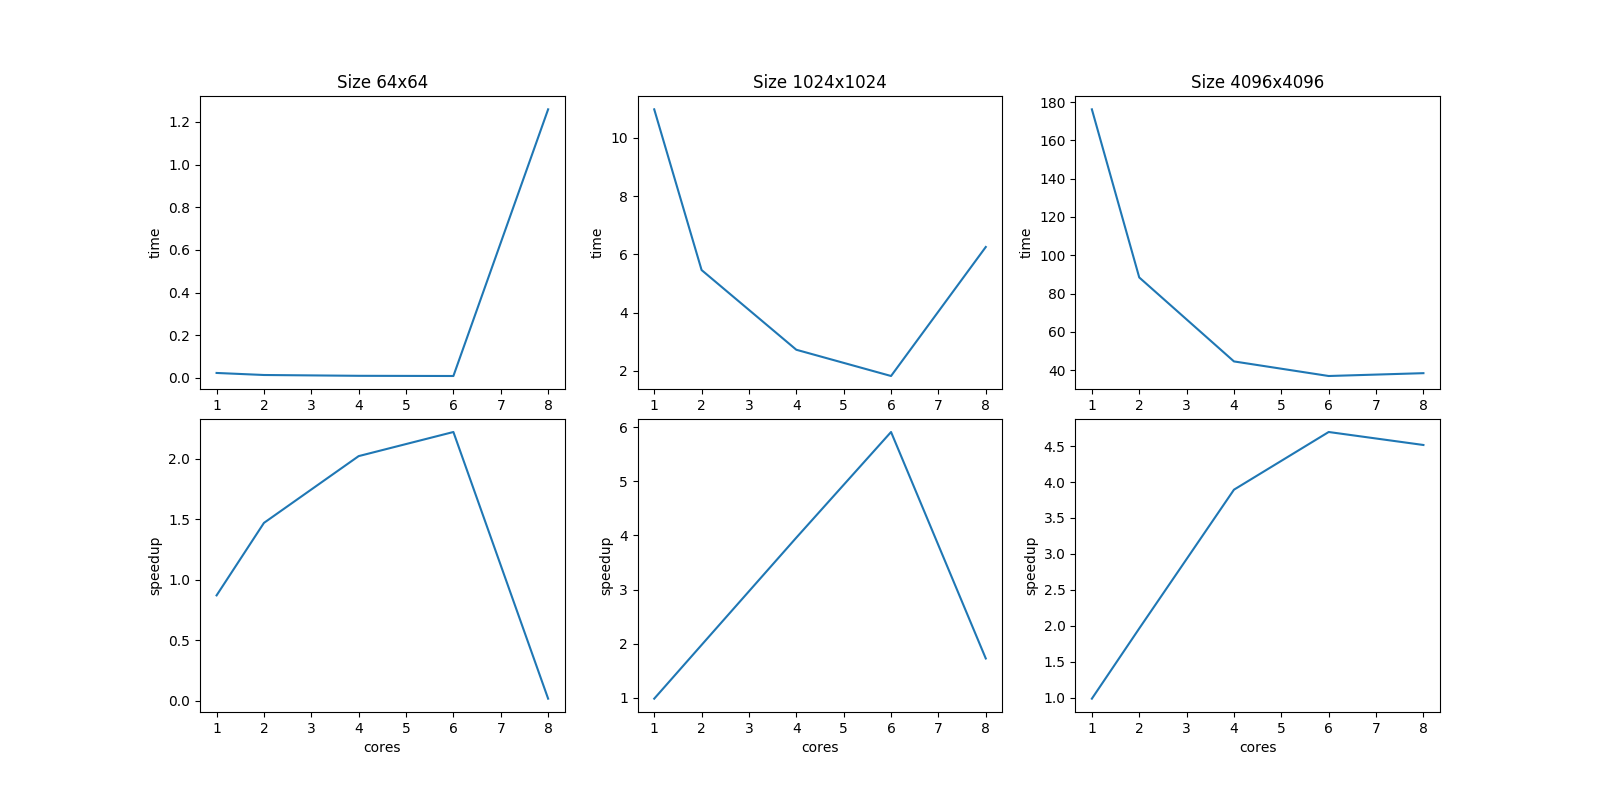
\includegraphics[width=16cm, height=8cm]{../3_images/plot.png}}
Παρατηρούμε ότι σε όλα τα μεγέθη του προβλήματος ο χρόνος πέφτει (και το \e{speedup} μεγάλωνει) μέχρι τους 6 επεξεργαστές. \\\\
Επομένως, το κόστος συγχρονισμού/επικοινωνίας και διαχείρισης των νημάτων
φαίνεται να υπερβαίνει το κέρδος της παραλληλοποίησης στους 8
επεξεραγαστές (σπάει η κλιμακωσιμότητα). Μάλιστα, στο \e{64x64} λόγω πολύ μικρού μεγέθους το φαινόμενο αυτό παίζει τόσο μεγάλο ρόλο που οι 8 επεξεργαστές έκαναν (εντυπωσιακά) πιο πολύ χρόνο από το σειριακό πρόγραμμα!

\newpage
\section{Στρατηγική Παραλληλοποίησης \e{Floyd-Warshall}}
\begin{center}
  \large{Θα δημιουργήσουμε 1 \e{task graph} για κάθε έκδοση του αλγορίθμου.}
\end{center}

\subsection{\e{Standard} Έκδοση}
Για την \e{standard} έκδοση το \e{task graph} είναι αυτό των διαφανειών όπου για κάθε \e{k} κάθε στοιχείο της γραμμής και της στήλης \e{k} εξαρτάται από το στοιχείο $A_{kk}$ και τα υπόλοιπα στοιχεία εξαρτώνται από στοιχεία της γραμμής και της στήλης \e{k}.\\
\begin{figure}[H]
  \centering
  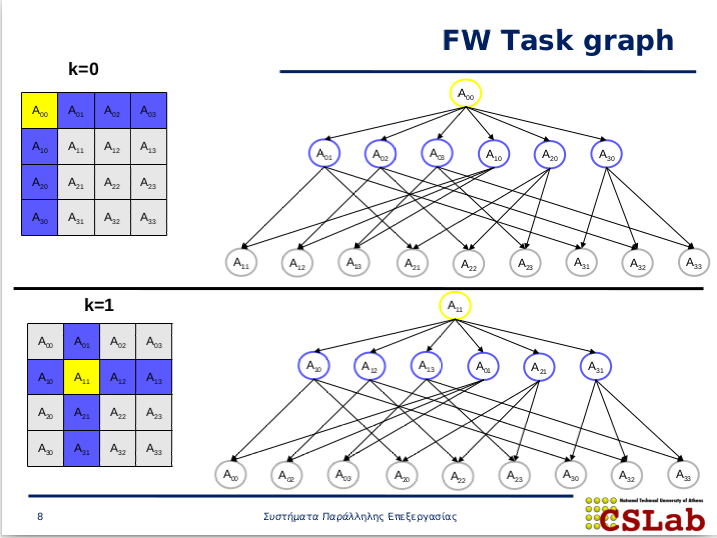
\includegraphics[width=10cm, height=8cm]{../3_images/fw.png}
  \caption{\e{Task graph standard} έκδοσης}
\end{figure}

\newpage
\subsection{\e{Recursive} Έκδοση}
Για την \e{recursive} έκδοση τα \e{tasks} είναι οι αναδρομικές κλήσεις. Στο σχήμα 2 έχουμε ένα \e{task graph} με κόμβους τα τεταρτημόρια στα οποία γράφει η αντίστοιχη αναδρομική κλήση και ένα όπου οι κόμβοι είναι το νούμερο της αναδρομικής κλήσεις με την σειρά που εμφανίζεται στον κώδικα.
\begin{figure}[H]
\centering
\begin{subfigure}{.35\textwidth}
  \centering
  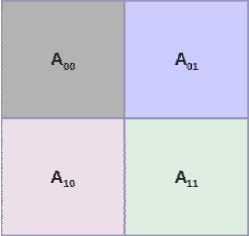
\includegraphics[width=.4\linewidth]{../3_images/recursive.png}
  \caption{Τεταρτημόρια}
  \label{fig:sub1}
\end{subfigure}%
\begin{subfigure}{.35\textwidth}
  \centering
  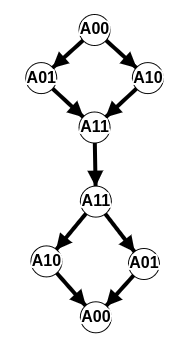
\includegraphics[width=.4\linewidth]{../3_images/recursivefw.png}
  \caption{\e{TG} με τεταρτημόρια}
  \label{fig:sub2}
\end{subfigure}%
\begin{subfigure}{.35\textwidth}
  \centering
  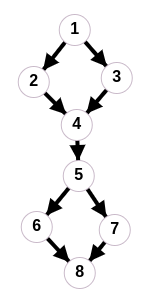
\includegraphics[width=.4\linewidth]{../3_images/recursivecalls.png}
  \caption{\e{TG} με νούμερα αναδρομικών κλήσεων}
  \label{fig:sub2}
\end{subfigure}
\caption{\e{Task graph recursive} έκδοσης}
\label{fig:test}
\end{figure}

\newpage
\subsection{\e{Tiled} Έκδοση}
Στην \e{tiled} έκδοση το \e{task graph} έχει την ίδια μορφή με εκείνο της \e{standard} έκδοσης, με την διαφορά ότι το A$_{ij}$ είναι το αντίστοιχο \e{block} και όχι απλά ένα στοιχείο του πίνακα.
\begin{figure}[H]
  \centering
  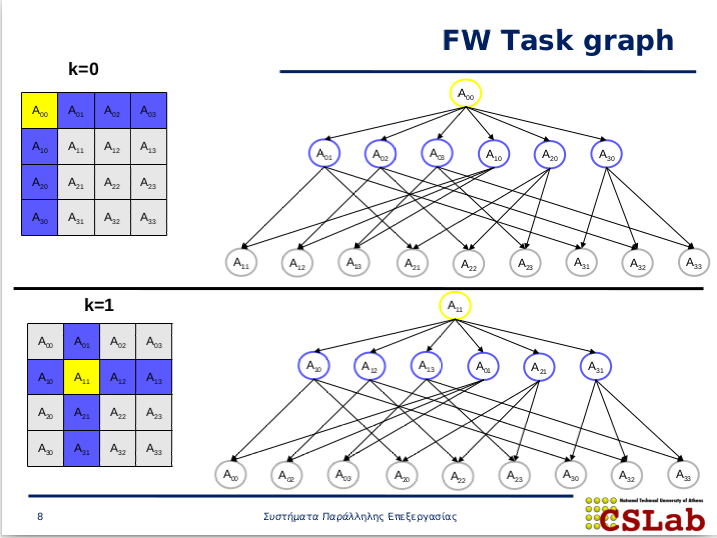
\includegraphics[width=10cm, height=8cm]{../3_images/fw.png}
  \caption{\e{Task graph tiled} έκδοσης}
\end{figure}

\end{document}
